\documentclass[10pt, twocolumn]{article}
\usepackage{amssymb,amsmath,latexsym, braket}
\usepackage{tikz, pgfplots, graphicx}
% Page length commands go here in the preamble
\setlength{\oddsidemargin}{-0.25in} % Left margin of 1 in + 0 in = 1 in
\setlength{\textwidth}{7in}   % Right margin of 8.5 in - 1 in - 6.5 in = 1 in
\setlength{\topmargin}{-.75in}  % Top margin of 2 in -0.75 in = 1 in
\setlength{\textheight}{9.2in}  % Lower margin of 11 in - 9 in - 1 in = 1 in


%\renewcommand{\baselinestretch}{1.5} % 1.5 denotes double spacing. Changing it will change the spacing

\setlength{\parindent}{0in} 

\begin{document}
\title{Review of Bell's theorem}
\author{Manish Goregaokar\\\small Affiliation: IIT Bombay}
\date{October 7, 2014}
\maketitle
\abstract{This paper gives an overview of a very important result from quantum mechanics; the Bell inequality and Bell's theorem. This theorem is what gives rise to the probabalisticness of quantum mechanics, disallowing interpretations that ascribe quantum effects to ignorance of local properties, i.e. local hidden variable theories. In this paper we analyse the theoretical foundation of the inequality and experimental backing of the same}
\setcounter{tocdepth}{2}
\tableofcontents
\section{Introduction}
In 1935, Einstein, Podolsky, and Rosen wrote their famous paper\cite{epr} which cast doubts on the completeness of quantum theory and its interoperability with special relativity. It described a process whichviolates the principle of local realism. Simply put, if two entangled particles are taken far apart, and one is observed, the state of the other particle is immediately collapsed. This is a ``spooky action at a distance" which violates the principle of locality, which Einstein et al found distasteful. Local hidden variable theories are those which prescribe that the state post-collapse is already determined pre-collapse, but is unknown to any observers. These resolve the EPR paradox, however are inconsistent with many quantum effects.\\

In 1964, John Bell proposed\cite{bell} an inequality concerning corellations that was satisfied for classical systems (with local realism), but was violated if the classical parameter was swapped for a quantum one like spin, proving that quantum systems do not obey local realism. This gives rise to Bell's theorem, \textbf{No physical theory of local hidden variables can ever reproduce all of the predictions of quantum mechanics}.\\
The inequality was later improved to remove the restriction that parallel measurement parameters should give anticorellated results in the 1969 paper\cite{chsh} by Clauser et al. The same paper first proposed a generic experimental setup (called "CHSH") for verifying the results. In Clauser and Horne's 1974 paper\cite{ch74}, the setup was refined to remove the dependency on fair sampling (called "CH74").\\

Experimentally, the first test of the Bell inequality was in 1972\cite{PhysRevLett.28.938}. Two more using the CH74 test were conducted in 1981-82 by Aspect et al\cite{PhysRevLett.47.460}\cite{PhysRevLett.49.1804}. The detection loophole was closed in 2001\cite{rowe2001experimental}.\\

Bell test experiments are still done to this day.

\section{Theoretical background}
\subsection{EPR paradox}
A concise explanation of the EPR paradox follows.

Alice and Bob are far away from each other. In between them, Eve carries out an experiment where a spin singlet state ($\Ket{\uparrow\downarrow}-\Ket{\downarrow\uparrow}$) is emitted. Eve sends one particle each to Alice and Bob.

Now, Bob makes a measurement along the $z$ axis, and gets the result (say) that the photon is aligned along the $+z$ axis. This collapses Alice's state to $\ket{\downarrow}$, since the projection of $\Ket{\uparrow\downarrow}-\Ket{\downarrow\uparrow}$ on the space $\Ket{\uparrow}\otimes\Ket{\phi}$ is $\Ket{\uparrow\downarrow}$.

The no-cloning theorem\cite{wootters1982single} prevents this from allowing usable superluminal communication (and thus does not generate any paradoxes in relativity), however it does violate the principle of local realism. Local space can now be affected by more than its immediate neighbors, which is the crux of this paradox.\\

\subsection{Hidden variable theories}
A way of circumventing the paradox is to propose hidden variable theories, where all states are ``predetermined", but ``hidden". In this case, the state would be predetermined to be $\Ket{\uparrow\downarrow}$ (In fact, we would need to predetermine a state for each of the three measurement directions), however physics would behave as if the state is probabalistic. This, however, requires an underlying theory of physics that resolves to quantum mechanics. As we shall see later in this report, hidden variable theories are an unlikely description of how the universe works.

\subsection{Quantum corellation}
An important concept for understanding Bell's theorem is quantum corellation.

Let us take a two state system with eigenvalues $\pm 1$. If we have an entangled pair of such systems, the quantum corellation is the expectation value of the product of the outcomes. If we take a large number $N$ of experiments, the quantum corellation becomes 
$$\frac{N_{++}-N_{+-}+N_{--}-N_{-+}}{N}$$

An important thing to note is that in an experiment there is bound to be a lot of noise in the observations. Hence while calculating quantum corellation, we must do so by first filtering out observations where there was no \textsl{coincidence}, using a \textsl{coincidence counter}. Such a device registers when both arms of the apparatus have made an observation and only then increments the relevant counters.

\subsection{Corellation for classical variables}
Let us consider a macroscopic object which explodes, giving rise to two fragments with opposite angular momenta (and opposite momenta). Observers $A$ and $B$ each observe the angular momentum (or momentum) $\vec j_A, \vec j_B$ of a single fragment each, along axes $\vec\alpha, \vec\beta$ respectively. $A$ calculates $s_A = \mathrm{sign}(\vec \alpha\cdot\vec j_A)$, and $B$ calculates $s_B$.\\

Note that if $\vec\alpha,\vec\beta$ are parallel, $s_A,s_B$ will have opposite signs, and vice versa. Generalizing a bit, if we know that $\vec\alpha,\vec\beta$ are parallel, the results will always be perfectly anticorellated ($\Braket{s_As_B}=-1$). (This assumption of the orientation of states is from Bell's original paper\cite{bell}, however it can be removed using formulae from the paper by Clauser et al\cite{chsh}). For arbitrary $\vec\alpha,\vec\beta$, the sphere of possible $\vec j_A$ values is divided into four parts by the two planes perpendicular to $\vec\alpha,\vec\beta$. These parts have areas in a ratio of $\theta:\pi-\theta:\theta:\pi-\theta$ for $N_{++}:N_{+-}:N_{--}:N_{++}$ ($\theta = \vec \alpha\angle\vec\beta$), giving us a corellation of 
\begin{align*}
\Braket{s_As_B} &= \frac{N_{++}-N_{+-}+N_{--}-N_{-+}}{N}\\
&= \frac{\theta-\pi+\theta+\theta -\pi +\theta}{2\pi}\\
&= 2\theta/\pi - 1
\end{align*}
\subsection{Corellation for quantum variables}
Instead of measuring macroscopic angular momentum, let us try measuring spin instead for spin-$\frac12$ particles.\\

Now, $\hat s_A=\vec\alpha\cdot\vec \sigma$, where $\vec \sigma$ is the Pauli matrix. $\hat s_b$ will have a negative sign since the spins are opposite.

\begin{align*}
\Braket{s_As_B} &= \Braket{(\vec\alpha\cdot\vec \sigma)(\vec\beta\cdot(-\vec \sigma))}\\
&= \Braket{-\alpha\cdot\beta}\\
&= -\cos{\theta}
\end{align*}
\begin{figure}

\begin{tikzpicture}
    \begin{axis}[domain=0:180,legend pos=south east,
    axis lines*=middle,
    xtick={90,180},
    xticklabels={$\frac{\pi}{2}$,$\pi$},
    xlabel=$\theta$,
    ylabel=$\Braket{s_As_B}$,
    every axis x label/.style={at={(current axis.right of origin)},anchor=north west},
    every axis y label/.style={at={(current axis.left of origin)},anchor=south east},
     axis lines = middle,]
    \addplot[mark=none, dashed] {-cos(x)}; 
    \addplot[mark=none] {x/90 - 1}; 
    \legend{Quantum,Classical}
    \end{axis}
\end{tikzpicture}
\caption{Variation of corellation with time. Note the differences between the classical and quantum cases}
\end{figure}
\section{Bell's inequality}
The following proof is adapted from Bell's original paper\cite{bell}\\

Let $\lambda$ be the predetermined "hidden variable" that is determined when the pair of states is formed. $s_A=s_A(\lambda), s_B=s_B(\lambda)$. Furthermore, let us allow ourselves to vary $\alpha, \beta$, so we deal with $s_A(\vec \alpha,\lambda), s_B(\vec \beta,\lambda)$. Let $\rho(\lambda)$ be the probability distribution of $\lambda$. What we will do is hypothetically orient $B$ in a different direction, and see what the result is. Some notation: $\Braket{s_A(\vec \alpha),s_B(\vec \beta)}=\Braket{\alpha,\beta}$

The expectation value for the product of the two observables should be:
\begin{align*}
\Braket{\alpha,\beta} &= \int \mathrm d \lambda\rho(\lambda) s_A(\vec \alpha,\lambda) s_B(\vec \beta,\lambda)\\
&= -\int \mathrm d \lambda\rho(\lambda) s_A(\vec \alpha,\lambda) s_A(\vec \beta,\lambda)\\
\therefore \Braket{\alpha,\beta} - \Braket{\alpha,\gamma} &= -\int \mathrm d \lambda\rho(\lambda)s_A(\vec \alpha,\lambda)(s_A(\vec \beta,\lambda) \\&\qquad- s_A(\vec\gamma,\lambda))\\
&=-\int \mathrm d \lambda\rho(\lambda)s_A(\vec \alpha,\lambda)(s_A(\vec \beta,\lambda) \\&\qquad - s_A(\vec\gamma,\lambda)s_A(\vec \beta,\lambda)^2)\\
&(\because s_A(\vec \beta,\lambda)=\pm 1)\\
&=-\int \mathrm d \lambda\rho(\lambda)s_A(\vec \alpha,\lambda)s_A(\vec \beta,\lambda)\\&\qquad(1 - s_A(\vec\gamma,\lambda)s_A(\vec \beta,\lambda))\\
\therefore \left|\Braket{\alpha,\beta} - \Braket{\alpha,\gamma}\right|&\leq -\int \mathrm d \lambda\rho(\lambda)(1 - s_A(\vec\gamma,\lambda)s_A(\vec \beta,\lambda))\\
&\because s_A = \pm 1\\
\therefore  \left|\Braket{\alpha,\beta} - \Braket{\alpha,\gamma}\right| &\leq \Braket{\beta, \gamma} - 1
\end{align*}

This is Bell's inequality. While it holds true for the classical case, for the case of spins we get $|\vec\alpha\cdot(\vec\beta-\vec\gamma)|\leq\vec\beta\cdot\vec\gamma - 1$, which is trivially untrue when $\vec\beta\angle\vec\gamma \geq \frac\pi2$.\\

This rules out the assumption of the ability for hidden variable theories to explain reality, as the existence of hidden variables was the only assumption in the derivation above.

\subsection{CHSH inequality}
The inequality above assumed that $s_B(\alpha,\lambda)=-s_A(\alpha,\lambda)$. This is not necessary for the general case, as shown by Clauser et al\cite{chsh}. The following is a proof adapted from Peres' paper\cite{teorema} on the subject.\\

By local realism, the results obtained by $A$ and $B$ should be independent of each other. If $B$ oriented his apparatus along a different direction $\vec\beta'$, $A$ would get the same results -- both $\Braket{s_A(\vec\alpha)}$ and $s_A(\vec\alpha)_i$ for each observation $i$ would be the same.

Now, since $s(x) = \pm 1$, $s_A(\alpha)s_B(\beta)+ s_A(\alpha')s_B(\beta)+ s_A(\alpha)s_B(\beta')-s_A(\alpha')s_B(\beta')=\pm 2$
$$\therefore \left|\frac{\sum s(\alpha)s(\beta)+ s(\alpha')s(\beta)+ s(\alpha)s(\beta')-s(\alpha')s(\beta')}{N}\right|\leq 2$$

Giving us $ \boxed{\left|\Braket{\alpha,\beta}+\Braket{\alpha',\beta}+\Braket{\alpha,\beta'}-\Braket{\alpha',\beta'}\right|\leq 2}$\\ which is the CHSH inequality. Once again, this is violated for the quantum case.

\subsection{Theoretical analysis}

There are multiple ways of resolving the paradox. One is to simply assume that unperformed experiments have no bearing on reality, thus rendering the detector settings $\alpha',\beta',\gamma$ superfluous (invalidating the basis of Bell's inequality).

Alternatively, we can take the stance that is most common today and simply discard local realism as a fundamental property of nature. This introduces some tension between quantum mechanics and non-quantum theories, however. For example, the wavefunction cannot be Lorentz invariant due to the instantaneous "action at a distance".
\section{Experimental background}
\subsection{Pile of plates polarizer}
A common apparatus here is a "pile of plates" polarizer. First, we choose a suitable birefringent material. When a birefringent material is subjected to unpolarized light at Brewster's angle, perfectly polarized light is reflected out, and slightly polarized light is refracted. On making a pile of such plates (Figure~\ref{fig:pop}), we get a polarizer that splits light into two polarizations perfectly.
\begin{figure}
\centering
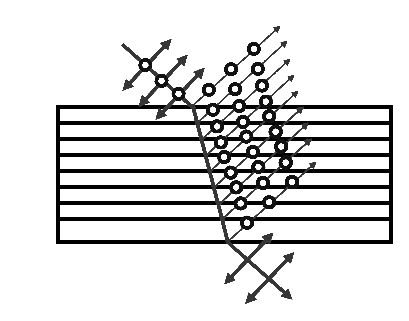
\includegraphics[scale=0.4]{pileofplates}
\caption{Pile of plates polarizer}
\label{fig:pop}
\end{figure}
\subsection{Parametric down conversion}
Parametric down conversion is the process used for creating entangled pairs of photons for most Bell test experiments. In this process, a material absorbs a photon and emits two photons of corellated polarizations (usually opposite) and with opposing momentum components in the perpendicular direction to the incident photon. One such material is a $\beta$-barium borate crystal\cite{PhysRevLett.75.4337}. 

This is a second order nonlinear process(Figure~\ref{fig:pdc}), caused by vacuum fluctuations in the crystal.

\begin{figure}
\centering
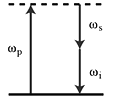
\includegraphics[scale=0.7]{pdc}
\caption{The process of parametric down conversion}
\label{fig:pdc}
\end{figure}

Sources typically use a laser pump to power the crystal.
\section{Experimental apparatus}
\subsection{Two-channel CHSH apparatus}
A typical two-channel CHSH apparatus (Figure~\ref{fig:chsh}) as used in \cite{PhysRevLett.49.91} consists of a source $S$, which emits photons with opposite polarizations. On either side there are two-channel polarizers which can be oriented to angle $a,b$. Each channel goes to a detector, which is wired back to a coincidence counter. The coincidence counter registers a reading only when one each of $D_+/D_-$ on either side simultaneously detects a photon. We use the CHSH inequality and calculate the corellation $\Braket{a,b}=\frac{N_{++} - N_{+-} + N_{--} - N_{-+}}{N_{++} + N_{+-} + N_{--} + N_{-+}}$. We now choose $a', b'$ and repeat the experiment for $\Braket{a',b},\Braket{a,b'},\Braket{a',b'}$. Finally, we calculate $S=\Braket{a,b}-\Braket{a,b'}+\Braket{a,b'}+\Braket{a',b'}$. If $|S|\geq 2$, local realism is refuted.

\begin{figure}
\centering
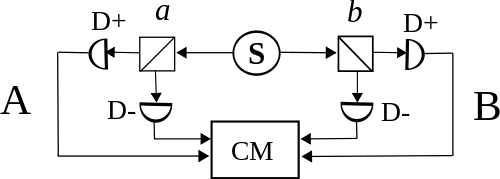
\includegraphics[scale=0.5]{chsh-2ch}
\caption{Two channel CHSH apparatus}
\label{fig:chsh}
\end{figure}

\subsection{Single channel CH74 apparatus}
Here, we use a single channel pile of plates polarizer (Figure~\ref{fig:ch74}), however in addition to the four experiments with different settings for either polarizer, we also have experiments where one or more polarizer is absent. We then calculate $S=\frac{\Braket{a,b}-\Braket{a,b'}+\Braket{a',b}+\Braket{a',b'}-\Braket{a',0}
-\Braket{0,b}}{\Braket{0,0}}$ where $0$ is used to denote the absence of a polarizer. $S>0$ is a violation of local realism.
\begin{figure}
\centering
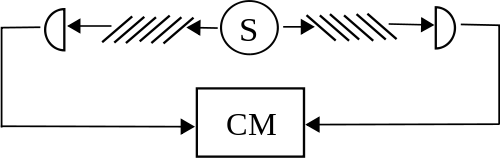
\includegraphics[scale=0.5]{ch74-1ch}
\caption{Single channel CH74 apparatus}
\label{fig:ch74}
\end{figure}

The existence of the $0$ readings lets us partially remove\cite{ch74} the "fair sampling" assumption.
\subsection{Loopholes}
There are a couple of common loopholes to Bell test experiments.

The fair sampling loophole points out that the sample of photons picked up by the detectors may not be representative of the entire generated sample. The detection loophole includes the fair sampling loophole, as well as cases where there is a double detection.\\

The communication loophole is due to our assumption that no communication occurs between the two detection sites. This loophole can be removed by increasing the distance between the sites such that no lightspeed communication can occur within the time of detection. However, most attempts to  do this decrease detection efficiency.\\

The disjoint sampling loophole deals with the fact that for parameter values $a',b',\gamma$, we did not carry out the \emph{same} experiment on the arm with the unchanged parameter, instead we carried out a new experiment, changing the actual values. This can be fixed if a suitable three-particle system can be found.

\subsection{Experimental history}
The first Bell test experiment was conducted in 1972 by Freedman and Clauser\cite{PhysRevLett.28.938}. Calcium atoms were heated to generate the photon pairs, with a single-channel apparatus.

The CHSH inequality was first used by Aspect et al\cite{PhysRevLett.49.1804}, using a two channel apparatus. This also used time varying analysers instead of restricting the parameter values. This used the same calcium excitation cascade as the previous experiment.

In 1994 an appreciable effort towards fixing the communication loophole was made by Tapster et al\cite{PhysRevLett.100.220404}, using  photon pairs generated by parametric down conversions and a lot of optical fiber.

In 2000, the disjoint sampling loophole was closed by Pan et al\cite{2000Natur.403..515P} using a three-particle Greenberger--Horne--Zeilinger\cite{2007arXiv0712.0921G} system.

In 2001, the detection loophole was closed for the first time by Rowe et al\cite{rowe2001experimental} using beryllium atoms coupled by a Raman transition using an apparatus described in \cite{sackett2000experimental}. This experiment is unfortunately very prone to the communication loophole.

In 2008 a major step towards plugging the communication loophole was made by Salart et al \cite{PhysRevLett.100.220404} with an 18km separation.

In 2013, the detection loophole was closed for photons\cite{giustina2013bell} using the Eberhard inequality\cite{eberhard1993background}
\section{Conclusion}
Bell's theorem is a cornerstone for quantum mechanics, which cements the probabalistic nature in place. While it can be escaped via metaphysical arguments (``experiments which do not occur do not count"), it is usually accepted as true and included in quantum interpretations. Experimental verification has been a resounding success for Bell's theorem, however there are still loopholes to be solved. Though the major loopholes have been individually plugged\cite{giustina2013bell}\cite{PhysRevLett.100.220404} for photons; there is still a lot of scope for formulating an experiment which simultaneously bypasses all loopholes.
\bibliographystyle{abbrv}
\bibliography{bib}

\end{document}